% ============================================================
%  Portfolio Optimization with Black-Litterman
%  A Case Study in Public Portfolio Disclosures
% ============================================================
\documentclass[aspectratio=169, 10pt]{beamer}

% ── Theme ──────────────────────────────────────────────────
\usetheme{Madrid}

% ── Custom palette colours ─────────────────────────────────
\definecolor{blnavy}{RGB}{26,  73, 101}   % deep navy
\definecolor{blamber}{RGB}{202,103,  2}   % amber accent
\definecolor{blteal}{RGB}{ 42,157, 143}   % teal accent
\definecolor{blgrey}{RGB}{245,245,245}    % slide background tint

\setbeamercolor{palette primary}   {bg=blnavy,       fg=white}
\setbeamercolor{palette secondary} {bg=blnavy!85,    fg=white}
\setbeamercolor{palette tertiary}  {bg=blnavy!65,    fg=white}
\setbeamercolor{palette quaternary}{bg=blnavy,       fg=white}
\setbeamercolor{structure}         {fg=blnavy}
\setbeamercolor{section in toc}    {fg=blnavy}
\setbeamercolor{alerted text}      {fg=blamber}
\setbeamercolor{block title}       {bg=blnavy,       fg=white}
\setbeamercolor{block body}        {bg=blnavy!8}
\setbeamercolor{block title alerted}{bg=blamber,     fg=white}
\setbeamercolor{block body alerted} {bg=blamber!10}

% ── Fonts & encoding ───────────────────────────────────────
\usepackage[T1]{fontenc}
\usepackage[utf8]{inputenc}
\usepackage{lmodern}

% ── Math ───────────────────────────────────────────────────
\usepackage{amsmath, amssymb, bm}

% ── Tables ─────────────────────────────────────────────────
\usepackage{booktabs}
\usepackage{array}
\usepackage{colortbl}
\newcolumntype{L}[1]{>{\raggedright\arraybackslash}p{#1}}
\newcolumntype{C}[1]{>{\centering\arraybackslash}p{#1}}

% ── Misc ───────────────────────────────────────────────────
\usepackage{microtype}
\usepackage{tikz}
\usetikzlibrary{arrows.meta, positioning, shapes.geometric}

% ── Metadata ───────────────────────────────────────────────
\title[BL Portfolio Optimization]{%
  Portfolio Optimization with Black-Litterman\\[4pt]
  \large A Case Study in Public Portfolio Disclosures}
\author{}
\date{}

% ── Helpers ────────────────────────────────────────────────
\newcommand{\tick}{\textcolor{blteal}{\textbullet}}
\newcommand{\BL}{\mathrm{BL}}

% ============================================================
\begin{document}
% ============================================================

% ── Title frame ─────────────────────────────────────────────
{
\setbeamertemplate{headline}{}
\begin{frame}[plain]
  \titlepage
  \vspace{-1.6em}
  \begin{center}
    \small
    \textcolor{blnavy!70}{
      Walk-forward backtest \(\cdot\) Real SEC \& congressional filing data \(\cdot\)
      Buffett \(\cdot\) Pelosi \(\cdot\) Trump}
  \end{center}
\end{frame}
}

% ── Agenda ──────────────────────────────────────────────────
\begin{frame}{Agenda}
  \tableofcontents
\end{frame}

% ============================================================
\section{Motivation \& Research Question}
% ============================================================

\begin{frame}{What Can Public Disclosures Tell Us?}

  \begin{columns}[T]
    \begin{column}{0.52\textwidth}
      \textbf{Three filing types, three portfolios}
      \medskip

      \begin{tabular}{@{}L{1.6cm} L{4.4cm}@{}}
        \toprule
        \textbf{Person} & \textbf{Filing source} \\
        \midrule
        Buffett  & SEC 13F (Berkshire Hathaway) \\[2pt]
        Pelosi   & U.S.\ House Financial Disclosure (FD)\\[2pt]
        Trump    & OGE 278e Annual Disclosure \\
        \bottomrule
      \end{tabular}
      \bigskip

      \begin{itemize}
        \item Holdings and approximate weights are \textbf{public record}
        \item Provides a tractable universe of \emph{real} investor views
        \item Range-based values converted to midpoints / lower bounds
      \end{itemize}
    \end{column}

    \begin{column}{0.44\textwidth}
      \begin{block}{Core Research Question}
        Can a Black-Litterman overlay improve portfolio
        quality relative to:\\[6pt]
        \quad (1) the \textbf{disclosed} portfolio itself?\\[4pt]
        \quad (2) a \textbf{mean-variance} (sample-estimated) baseline?
      \end{block}
      \bigskip
      \textit{Improvement} is measured on risk-adjusted return,
      maximum drawdown, concentration (HHI), and turnover.
    \end{column}
  \end{columns}
\end{frame}

% ============================================================
\section{Data Pipeline}
% ============================================================

\begin{frame}{Data Pipeline}

  \begin{center}
  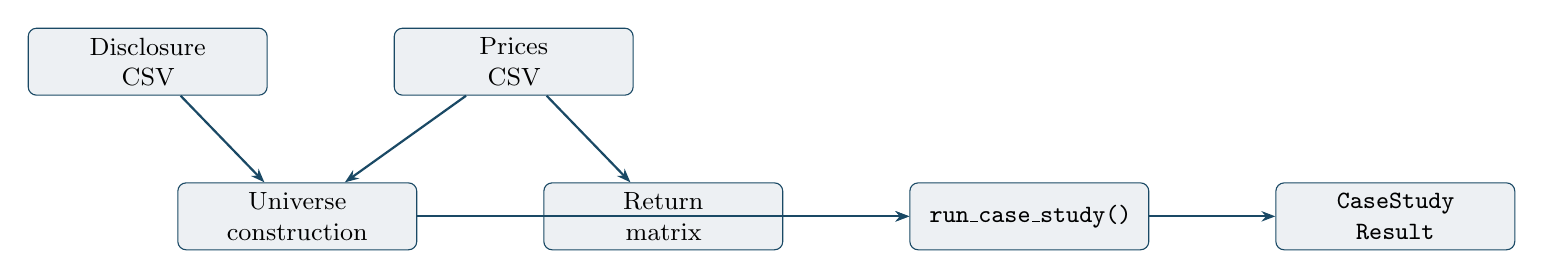
\begin{tikzpicture}[
      node distance=1.1cm and 1.6cm,
      box/.style={draw=blnavy, rounded corners=3pt,
                  fill=blnavy!8, text width=2.8cm,
                  align=center, minimum height=0.85cm, font=\small},
      arr/.style={-{Stealth[length=5pt]}, blnavy, thick}
    ]
    \node[box] (disc) {Disclosure\\CSV};
    \node[box, right=of disc] (prices) {Prices\\CSV};
    \node[box, below=of disc, xshift=1.9cm] (univ) {Universe\\construction};
    \node[box, right=of univ] (ret)  {Return\\matrix};
    \node[box, right=of ret]  (pipe) {\texttt{run\_case\_study()}};
    \node[box, right=of pipe] (res)  {\texttt{CaseStudy\\Result}};

    \draw[arr] (disc)   -- (univ);
    \draw[arr] (prices) -- (univ);
    \draw[arr] (prices) -- (ret);
    \draw[arr] (univ)   -- (pipe);
    \draw[arr] (ret)    -- (pipe);
    \draw[arr] (pipe)   -- (res);
  \end{tikzpicture}
  \end{center}

  \bigskip
  \begin{columns}[T]
    \begin{column}{0.48\textwidth}
      \textbf{Disclosures} (\texttt{data/disclosures.py})
      \begin{itemize}\small
        \item Schema validation on load
        \item Drops rows with missing/non-positive weight
        \item \texttt{latest\_portfolio\_for\_aliases()} selects the most recent filing
      \end{itemize}
    \end{column}
    \begin{column}{0.48\textwidth}
      \textbf{Prices} (\texttt{data/prices.py})
      \begin{itemize}\small
        \item 46 tickers, 2018-01-02 – 2025-12-30
        \item Split/dividend-adjusted daily closes (Yahoo Finance)
        \item Duplicate \texttt{(date, ticker)} pairs detected and warned
      \end{itemize}
    \end{column}
  \end{columns}
\end{frame}

% ============================================================
\section{Three Strategies}
% ============================================================

\begin{frame}{Three Strategies Compared}

  \begin{columns}[T]
    \begin{column}{0.31\textwidth}
      \begin{block}{\centering Disclosed}
        \centering\small
        Static buy-and-hold of the\\
        filed portfolio weights.\\[6pt]
        No rebalancing; zero turnover.\\[6pt]
        \textit{Upper bound on what a\\
        passive follower achieves.}
      \end{block}
    \end{column}

    \begin{column}{0.31\textwidth}
      \begin{block}{\centering Mean-Variance}
        \centering\small
        Long-only Markowitz on the\\
        same universe.\\[6pt]
        Sample mean \& covariance\\
        estimated over lookback window.\\[6pt]
        \textit{Classical quantitative\\
        benchmark.}
      \end{block}
    \end{column}

    \begin{column}{0.31\textwidth}
      \begin{alertblock}{\centering Black-Litterman}
        \centering\small
        Equilibrium prior blended\\
        with disclosure-implied views.\\[6pt]
        Posterior fed into long-only\\
        Markowitz optimiser.\\[6pt]
        \textit{Primary strategy\\
        under investigation.}
      \end{alertblock}
    \end{column}
  \end{columns}

  \bigskip
  \begin{center}
    \small All three strategies share the same universe, lookback window,\\
    rebalance schedule, and risk constraints — ensuring a fair comparison.
  \end{center}
\end{frame}

% ============================================================
\section{The Black-Litterman Model}
% ============================================================

\begin{frame}{Black-Litterman: Equilibrium Prior}

  \begin{columns}[T]
    \begin{column}{0.52\textwidth}

      \textbf{Step 1 — implied equilibrium returns}
      \[
        \bm{\pi} = \lambda\,\bm{\Sigma}\,\bm{w}_{\text{mkt}}
      \]

      \medskip
      \begin{tabular}{@{}cl@{}}
        $\lambda$ & risk-aversion scalar (default: $2.5$) \\
        $\bm{\Sigma}$ & sample covariance of asset returns \\
        $\bm{w}_{\text{mkt}}$ & market-cap proxy weights \\[4pt]
        $\bm{\pi}$ & equilibrium excess return vector \\
      \end{tabular}

      \bigskip
      \textbf{Step 2 — view matrix from disclosures}\\[4pt]
      Disclosed portfolio weights define a single \emph{absolute view}:
      \[
        P\bm{\mu} = \bm{q}, \qquad
        \bm{\Omega} = \frac{1 - c}{c}\,P\bm{\Sigma}P^{\top}
      \]
      where $c \in (0,1)$ is \textbf{view\_confidence} (default: $0.65$).
    \end{column}

    \begin{column}{0.44\textwidth}
      \begin{block}{Intuition}
        \small
        $c \to 1$: posterior collapses to the disclosed view.\\[4pt]
        $c \to 0$: posterior collapses to the equilibrium prior.\\[4pt]
        The sensitivity notebook sweeps $c \in [0.20,\,0.95]$
        across all three case studies ($16 \times 3 = 48$ backtests).
      \end{block}

      \bigskip
      \begin{block}{Why not pure MV on disclosures?}
        \small
        Sample-estimated means are notoriously noisy.
        The equilibrium prior \emph{regularises} expected returns
        before the disclosure signal is injected.
      \end{block}
    \end{column}
  \end{columns}
\end{frame}

\begin{frame}{Black-Litterman: Posterior Update}

  \textbf{Posterior precision matrix}
  \[
    M \;=\; (\tau\bm{\Sigma})^{-1} \;+\; P^{\top}\bm{\Omega}^{-1}P
  \]

  \textbf{Posterior mean returns}
  \[
    \bm{\mu}_{\BL} \;=\; M^{-1}
      \Bigl[(\tau\bm{\Sigma})^{-1}\bm{\pi} \;+\; P^{\top}\bm{\Omega}^{-1}\bm{q}\Bigr]
  \]

  \textbf{Posterior covariance}
  \[
    \bm{\Sigma}_{\BL} \;=\; \bm{\Sigma} \;+\; M^{-1}
  \]

  \medskip
  \begin{columns}[T]
    \begin{column}{0.48\textwidth}
      \begin{tabular}{@{}cl@{}}
        \toprule
        \textbf{Symbol} & \textbf{Meaning} \\
        \midrule
        $\tau$         & prior uncertainty scalar (default: $0.05$) \\
        $P$            & $k \times n$ view-picking matrix \\
        $\bm{q}$       & $k$-vector of view returns \\
        $\bm{\Omega}$  & $k \times k$ view uncertainty matrix \\
        \bottomrule
      \end{tabular}
    \end{column}

    \begin{column}{0.48\textwidth}
      \begin{alertblock}{Then: long-only Markowitz}
        \small
        $(\bm{\mu}_{\BL},\,\bm{\Sigma}_{\BL})$ are passed to a
        quadratic programme with $\bm{w} \ge 0$,\; $\mathbf{1}^{\top}\bm{w}=1$.\\[4pt]
        Falls back to equal-weight if the solver returns
        all non-positive weights.
      \end{alertblock}
    \end{column}
  \end{columns}
\end{frame}

% ============================================================
\section{Walk-Forward Backtest Engine}
% ============================================================

\begin{frame}{Walk-Forward Backtest Engine}

  \begin{columns}[T]
    \begin{column}{0.5\textwidth}
      \textbf{No-lookahead-bias design}
      \begin{itemize}
        \item Weights computed on data up to rebalance date $t$
        \item Applied to returns \emph{from the period after} $t$
        \item \texttt{weight\_history} indexed by decision date
      \end{itemize}

      \bigskip
      \textbf{Configuration} (YAML-driven)
      \medskip

      \begin{tabular}{@{}ll@{}}
        \toprule
        Parameter & Value \\
        \midrule
        \texttt{lookback\_periods}   & 6 months \\
        \texttt{rebalance\_frequency}& Month-end \\
        \texttt{risk\_aversion}      & $\lambda = 2.5$ \\
        \texttt{tau}                 & $\tau = 0.05$ \\
        \texttt{view\_confidence}    & $c = 0.65$ \\
        \bottomrule
      \end{tabular}
    \end{column}

    \begin{column}{0.46\textwidth}
      \begin{block}{\texttt{rolling\_backtest()} flow}
        \small
        \begin{enumerate}
          \item Slice price history to lookback window
          \item Compute return matrix
          \item Call weight function (BL / MV / static)
          \item On failure: fall back to equal-weight \& warn
          \item Accumulate: NAV, returns, weight history
        \end{enumerate}
      \end{block}

      \bigskip
      \begin{block}{Output: \texttt{BacktestResult}}
        \small
        \texttt{.returns} \quad daily return series\\
        \texttt{.nav} \quad \phantom{dai}cumulative NAV\\
        \texttt{.weight\_history} \quad rebalance weights
      \end{block}
    \end{column}
  \end{columns}
\end{frame}

% ============================================================
\section{Performance Metrics}
% ============================================================

\begin{frame}{Performance Metrics Suite}

  \begin{columns}[T]
    \begin{column}{0.48\textwidth}
      \textbf{Return \& risk}
      \medskip

      \begin{tabular}{@{}L{3.2cm} L{4.2cm}@{}}
        \toprule
        Metric & Notes \\
        \midrule
        Annual return    & Geometric compounding \\
        Annual volatility& Annualised std dev \\
        Sharpe ratio     & Excess return / vol \\
        Sortino ratio    & Returns \texttt{nan} (not $+\infty$) when no downside exists \\
        Max drawdown     & Peak-to-trough NAV \\
        \bottomrule
      \end{tabular}
    \end{column}

    \begin{column}{0.48\textwidth}
      \textbf{Portfolio quality}
      \medskip

      \begin{tabular}{@{}L{3.2cm} L{4.2cm}@{}}
        \toprule
        Metric & Notes \\
        \midrule
        HHI concentration & $\sum w_i^2$; higher = more concentrated \\
        Average turnover  & Mean $L_1$ weight change per rebalance \\
        \bottomrule
      \end{tabular}

      \bigskip
      \begin{block}{Frequency inference}
        \small
        \texttt{infer\_periods\_per\_year()} detects
        daily / monthly / quarterly frequency
        automatically from the return index.
        Emits a \texttt{UserWarning} when fewer
        than 3 observations are available.
      \end{block}
    \end{column}
  \end{columns}
\end{frame}

% ============================================================
\section{Notebooks \& Results}
% ============================================================

\begin{frame}{Four Analysis Notebooks}

  \begin{tabular}{@{}C{0.4cm} L{5cm} L{8.2cm}@{}}
    \toprule
    \textbf{\#} & \textbf{Title} & \textbf{What you see} \\
    \midrule
    1 & Data Quality \& Universe Overview
      & Schema checks, holdings coverage, disclosed portfolio composition
        and pie charts — for all three persons \\[6pt]
    2 & Strategy Comparison Case Study
      & Equity curves, drawdown charts, BL weight evolution,
        and combined summary table — for all three persons \\[6pt]
    3 & BL Sensitivity Analysis
      & 48-run confidence sweep ($c \in [0.20, 0.95]$, 16 values $\times$ 3 persons);
        2$\times$3 subplot grid: return, vol, Sharpe, HHI, turnover vs.\ $c$ \\[6pt]
    4 & Benchmark Attribution \& Alpha Decomposition
      & OLS factor model (SPY, Tech, Energy, Financials, ConsumerDisc);
        beta table, contribution bars, rolling 12-month $\alpha$/$\beta$ \\
    \bottomrule
  \end{tabular}

  \bigskip
  \begin{center}
    \small All notebooks loop over \textbf{Buffett}, \textbf{Pelosi}, and \textbf{Trump}
    from a shared \texttt{results} dict --- no hardcoded person keys.
  \end{center}
\end{frame}

\begin{frame}{Notebook 03 — Sensitivity to View Confidence}

  \begin{columns}[T]
    \begin{column}{0.5\textwidth}
      \textbf{What the sweep reveals}
      \begin{itemize}
        \item Sharpe is \emph{non-monotonic} in $c$ on real data —
              the ``optimal'' confidence differs by person
        \item Higher $c$ $\Rightarrow$ increased turnover when views
              diverge from equilibrium
        \item HHI spikes near extreme confidence values,
              indicating concentrated allocation
      \end{itemize}

      \bigskip
      \textbf{Practical use}\\
      The sweep provides a principled starting range for
      \texttt{view\_confidence} before out-of-sample reporting.
      The best-by-Sharpe row is printed per person.
    \end{column}

    \begin{column}{0.46\textwidth}
      \begin{block}{Sweep configuration}
        \small
        \begin{tabular}{@{}ll@{}}
          Grid       & $c \in \{0.20, 0.25, \ldots, 0.95\}$ \\
          Points     & 16 per person \\
          Persons    & 3 (Buffett, Pelosi, Trump) \\
          \midrule
          Total runs & \textbf{48 backtests} \\
        \end{tabular}
      \end{block}

      \bigskip
      \begin{block}{Colour scheme (all metric plots)}
        \small
        \textcolor{blnavy}{$\bullet$}\; Buffett \quad
        \textcolor{blamber}{$\bullet$}\; Pelosi \quad
        \textcolor{blteal}{$\bullet$}\; Trump \\[4pt]
        2$\times$3 subplot grid; 5 metrics shown,
        6th panel hidden.
      \end{block}
    \end{column}
  \end{columns}
\end{frame}

\begin{frame}{Notebook 04 — Benchmark Attribution}

  \textbf{OLS factor model}
  \[
    r_{\text{strat},t} = \alpha
      + \beta_1 r_{\text{SPY},t}
      + \beta_2 r_{\text{Tech},t}
      + \beta_3 r_{\text{Energy},t}
      + \beta_4 r_{\text{Fin},t}
      + \beta_5 r_{\text{CD},t}
      + \varepsilon_t
  \]

  \medskip
  \begin{columns}[T]
    \begin{column}{0.48\textwidth}
      \textbf{Benchmark panel construction}
      \begin{itemize}\small
        \item Prefers ETF tickers: SPY, XLK, XLE, XLF, XLY
        \item Falls back to explicit ticker proxies
          (e.g.\ AAPL+MSFT+NVDA for Tech) if ETFs absent
        \item Source provenance table printed per person
      \end{itemize}

      \bigskip
      \textbf{Output per person}
      \begin{itemize}\small
        \item $\hat{\beta}$ bar chart (positive = teal, negative = red)
        \item Annualised arithmetic contribution decomposition
        \item Return correlation heatmap
        \item Rolling 12-month $\hat{\alpha}$ and $\hat{\beta}$ vs.\ SPY
      \end{itemize}
    \end{column}

    \begin{column}{0.48\textwidth}
      \begin{block}{Attribution decomposition (arithmetic)}
        \small
        \[
          \bar{r}_{\text{ann}}
            \approx \underbrace{\hat{\alpha} \cdot f}_{\text{alpha contrib}}
            + \underbrace{\sum_k \hat{\beta}_k \bar{r}_{k,\text{ann}}}_{\text{factor contrib}}
            + \text{residual}
        \]
        where $f$ = periods per year.
      \end{block}

      \bigskip
      \begin{block}{Rolling diagnostics}
        \small
        12-month rolling OLS on strategy vs.\ SPY reveals
        \emph{regime shifts} hidden in full-sample statistics —
        particularly the 2020 COVID drawdown and 2022 rate shock.
      \end{block}
    \end{column}
  \end{columns}
\end{frame}

% ============================================================
\section{Codebase Architecture}
% ============================================================

\begin{frame}[fragile]{Codebase Architecture}

  \begin{columns}[T]
    \begin{column}{0.44\textwidth}
      \textbf{Package layout}
      \medskip
      \begin{tabular}{@{}L{3.8cm} L{3.6cm}@{}}
        \toprule
        Module & Responsibility \\
        \midrule
        \texttt{config.py}            & YAML loading, dataclasses \\
        \texttt{pipeline.py}          & \texttt{run\_case\_study()} \\
        \texttt{data/disclosures.py}  & Load \& validate holdings \\
        \texttt{data/prices.py}       & Load prices, pivot matrix \\
        \texttt{models/black\_litterman.py} & BL posterior \\
        \texttt{models/mean\_variance.py}   & Long-only Markowitz \\
        \texttt{backtest/engine.py}   & Rolling walk-forward \\
        \texttt{backtest/metrics.py}  & All performance metrics \\
        \bottomrule
      \end{tabular}
    \end{column}

    \begin{column}{0.52\textwidth}
      \textbf{Quality \& observability}
      \begin{itemize}
        \item \textbf{63 tests} — unit and integration
              (\texttt{pytest --tb=short})
        \item \texttt{logging.getLogger(\_\_name\_\_)} in every module;
              \texttt{--verbose} flag for \textsc{debug} output
        \item \texttt{FileNotFoundError} / \texttt{ValueError} raised
              with descriptive messages on bad inputs
        \item \texttt{\_\_all\_\_} exports defined in all
              \texttt{\_\_init\_\_.py} files
        \item \texttt{view\_confidence} and all BL hyperparameters
              exposed via YAML — no hardcoded magic numbers
      \end{itemize}

      \bigskip
      \textbf{CLI quick-start}
      \begin{verbatim}
PYTHONPATH=src python \
  scripts/run_case_study.py \
  --config configs/case_studies.yaml \
  --person buffett --verbose
      \end{verbatim}
    \end{column}
  \end{columns}
\end{frame}

% ============================================================
\section{Known Limitation \& Extensions}
% ============================================================

\begin{frame}{Known Model Limitation}

  \begin{alertblock}{Gaussian Prior Assumption}
    The BL posterior assumes multivariate Gaussianity in both returns and views.
    Equity return distributions exhibit significant \textbf{excess kurtosis} and
    \textbf{left-tail asymmetry}, particularly during stress periods directly
    visible in this backtest — the \textbf{2020 COVID drawdown} and the
    \textbf{2022 rate shock}.
  \end{alertblock}

  \bigskip
  \begin{columns}[T]
    \begin{column}{0.48\textwidth}
      \textbf{What this means in practice}
      \begin{itemize}
        \item Posterior covariance underestimates tail risk
        \item Optimiser over-allocates to assets that appear
              low-vol under normality but fat-tail in crises
        \item Sortino ratio and max drawdown metrics
              are the most informative diagnostics here
      \end{itemize}
    \end{column}

    \begin{column}{0.48\textwidth}
      \textbf{Production-grade alternative}
      \begin{itemize}
        \item Meucci's \textbf{Entropy Pooling} / Copula Opinion Pooling
        \item Separates marginal distributions from the
              dependence structure
        \item Allows views on \emph{arbitrary statistics}
              (e.g.\ implied volatility, tail quantiles)
        \item No Gaussian assumption required
      \end{itemize}
    \end{column}
  \end{columns}
\end{frame}

% ============================================================
\section{Summary}
% ============================================================

\begin{frame}{Summary}

  \begin{columns}[T]
    \begin{column}{0.48\textwidth}
      \textbf{What the framework provides}
      \begin{itemize}
        \item End-to-end walk-forward backtest on \emph{real}
              publicly-filed portfolio data
        \item Fair three-way strategy comparison:
              Disclosed / Mean-Variance / Black-Litterman
        \item Full sensitivity analysis over the key
              BL hyperparameter ($c$)
        \item OLS attribution with rolling diagnostics
        \item YAML-configurable — swap in any universe
              or parameter set without code changes
      \end{itemize}
    \end{column}

    \begin{column}{0.48\textwidth}
      \textbf{Key design decisions}
      \begin{itemize}
        \item No-lookahead-bias by construction
        \item Graceful degradation: equal-weight fallback
              with logged warning
        \item \texttt{nan} (not $+\infty$) Sortino on
              all-positive return periods
        \item Real adjusted prices via Yahoo Finance
              (2018 – 2025, 46 tickers)
        \item 63 tests enforce correctness at every layer
      \end{itemize}

      \bigskip
      \begin{block}{Limitation acknowledged}
        \small
        Gaussian prior — visible in 2020 \& 2022 stress
        periods. Entropy Pooling is the natural upgrade path.
      \end{block}
    \end{column}
  \end{columns}

  \vfill
  \begin{center}
    \textcolor{blnavy!60}{\rule{0.8\textwidth}{0.4pt}}\\[4pt]
    \small\textcolor{blnavy!70}{
      \texttt{github.com/mengrenman/portfolio-optimization-black-litterman}}
  \end{center}
\end{frame}

% ============================================================
\end{document}
% ============================================================
